\documentclass[border=10pt]{standalone}
\usepackage{tikz}
\usepackage[utf8]{inputenc}
\usepackage[T1]{fontenc}
\usetikzlibrary{patterns,arrows.meta}

\begin{document}

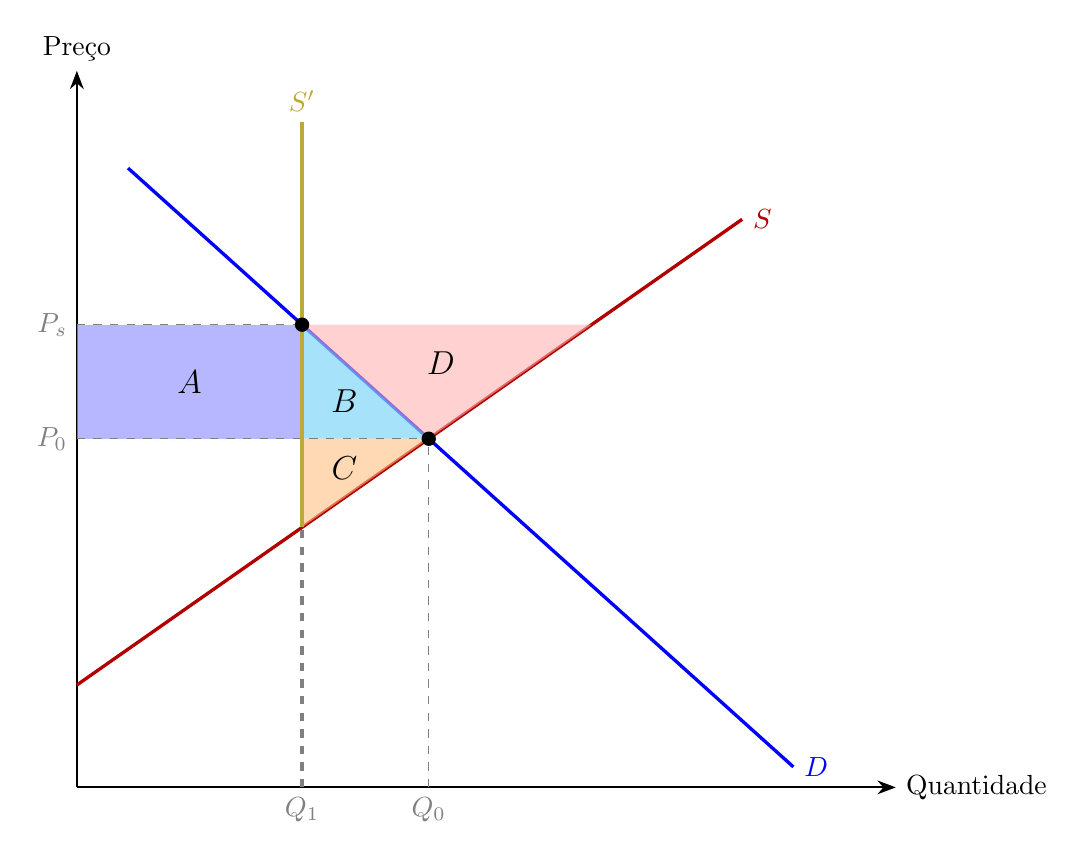
\begin{tikzpicture}[scale=1.3, >=Stealth]
    
    % Eixos
    \draw[thick,->] (0,0) -- (8,0) node[right] {Quantidade};
    \draw[thick,->] (0,0) -- (0,7) node[above] {Preço};
    
    % Curvas de oferta e demanda
    \draw[blue, very thick, domain=0.5:7] plot (\x, {6.5 - 0.9*\x}) node[right] {$D$};
    \draw[red!70!black, very thick, domain=0:6.5] plot (\x, {1.0 + 0.7*\x}) node[right] {$S$};
    
    % Coordenadas importantes
    \def\Ql{2.2}        % Quantidade limitada
    % Calcular equilíbrio: D = S => 6.5 - 0.9*x = 1.0 + 0.7*x
    % 5.5 = 1.6*x => x = 3.4375, y = 1.0 + 0.7*3.4375 = 3.406
    \def\Qeq{3.4375}    % Quantidade de equilíbrio
    \def\Peq{3.406}     % Preço de equilíbrio
    \def\Ps{4.52}       % Preço com oferta restrita
    
    % Área A (perda excedente do consumidor - azul)
    \fill[blue!40, opacity=0.7] (0,\Ps) -- (0,\Peq) -- (\Ql,\Peq) -- (\Ql,\Ps) -- cycle;
    
    % Área B (transferência - azul-verde)
    \fill[cyan!50, opacity=0.7] (\Ql,\Ps) -- (\Ql,\Peq) -- (\Qeq,\Peq) -- cycle;
    
    % Área C (perda excedente do produtor) - acima de S, abaixo de P0, de Q1 até Q0
    % Vértices: (Q1, na curva S), (Q1, P0), (Q0, P0)
    % S em Q1=2.2: y = 1.0 + 0.7*2.2 = 2.54
    \fill[orange!50, opacity=0.6] (\Ql,{1.0 + 0.7*\Ql}) -- (\Ql,\Peq) -- (\Qeq,\Peq) -- cycle;
    
    % Área D (perda de peso morto) - ABAIXO de Ps e ACIMA das curvas S e D
    % S em Ps=4.52: 4.52 = 1.0 + 0.7*x => x = 5.03
    % Vértices: (Q1, Ps), (Q0, P0), (5.03, Ps)
    \fill[red!30, opacity=0.6] (\Ql,\Ps) -- (\Qeq,\Peq) -- (5.03,\Ps) -- cycle;
    
    % Linhas tracejadas horizontais
    \draw[dashed, gray] (0,\Ps) node[left] {$P_s$} -- (\Ql,\Ps);
    \draw[dashed, gray] (0,\Peq) node[left] {$P_0$} -- (\Qeq,\Peq);
    
    % Linhas tracejadas verticais
    \draw[dashed, gray] (\Ql,0) node[below] {$Q_1$} -- (\Ql,\Ps);
    \draw[dashed, gray] (\Qeq,0) node[below] {$Q_0$} -- (\Qeq,\Peq);
    
    % Rótulos das áreas
    % Área A: retângulo (0, 3.406) a (2.2, 4.52) - centro: (1.1, 3.963)
    \node at (1.1, 3.963) {\large $A$};
    % Área B: triângulo (2.2, 4.52), (2.2, 3.406), (3.4375, 3.406) - centro: (2.613, 3.777)
    \node at (2.613, 3.777) {\large $B$};
    % Área C: triângulo (2.2, 2.54), (2.2, 3.406), (3.4375, 3.406) - centro: (2.613, 3.117)
    \node at (2.613, 3.117) {\large $C$};
    % Área D: triângulo (2.2, 4.52), (3.4375, 3.406), (5.03, 4.52) - centro: (3.556, 4.149)
    \node at (3.556, 4.149) {\large $D$};
    
    % Oferta restrita (linha vertical) - desenhar por último para sobrepor
    % S' é vertical em Q1=2.2, vai até onde toca S
    % S em x=2.2: y = 1.0 + 0.7*2.2 = 2.54
    \draw[dashed, gray, very thick] (2.2, 0) -- (2.2, 2.54);
    \draw[yellow!80!orange!70!black, very thick] (2.2, 2.54) -- (2.2, 6.5) node[above] {$S'$};
    
    % Ponto de equilíbrio
    \fill (\Qeq,\Peq) circle (2pt);
    
    % Ponto de interseção S' com D
    \fill (\Ql,\Ps) circle (2pt);
    
\end{tikzpicture}

\end{document}
